\index{magma}
Pohyby magmatu ze zemského pláště do zemské kůry mají za následek celou řadu forem reliéfu. V případě, že se magma dostává na povrch, jedná se o \textbf{extruzivní} magmatismus.  \textbf{Intruzivní} magmatismus dává za vznik formám reliéfu, které jsou patrné až po jejich obnažení.

\section{Formy reliéfu spojené s intruzemi magmatu}
\subsection{Velká intruzivní tělesa}
Mezi rozsáhlá intruzivní tělesa patří \textbf{batolity}, neboli také \textbf{plutony}. Tvoří je granitoidní horniny. Batolity jsou často v podloží nejvyšších částí kontinentálních orogénů. Intruze magmatu a vznik batolitu může způsobit vyklenutí nadložních sedimentárních hornin. Po exhumaci batolitu erozí nadložních hornin dochází k jeho zvětrávání podél puklin, které jsou organizované zpravidla do třech na sebe kolmých systémů. Obnažení intruzivních těles vede k uvolnňování napětí v hornině a vzniku sekundárních (exfoliačních) puklinových systémů. \textbf{Lopolit} je dalším typem rozsáhlého intruzivního tělesa. Má tvar pánve a je tvořeno bazickými horninami typu gabro. Telěso menšího rozsahu než batolit je \textbf{peň}.

\subsection{Intruzivní tělesa menšího rozměru}
Menší intruzivní tělesa doprovázejí větší intruzivní tělesa či extrusivní tělesa. Můžeme je rozdělit na konkordantní pokud probíhají podél původních vrstevních ploch a na diskordantní v případě jejich protnutí. Mezi diskordantní tělesa patří \textbf{pravé žíly} (Obr. \ref{fig:zila}). Jedná se o \SIrange{1}{10}{\metre} široká tělesa. Vyskytují se nejčastěji ve větších skupinách.

\begin{figure}[h]
	\centering
	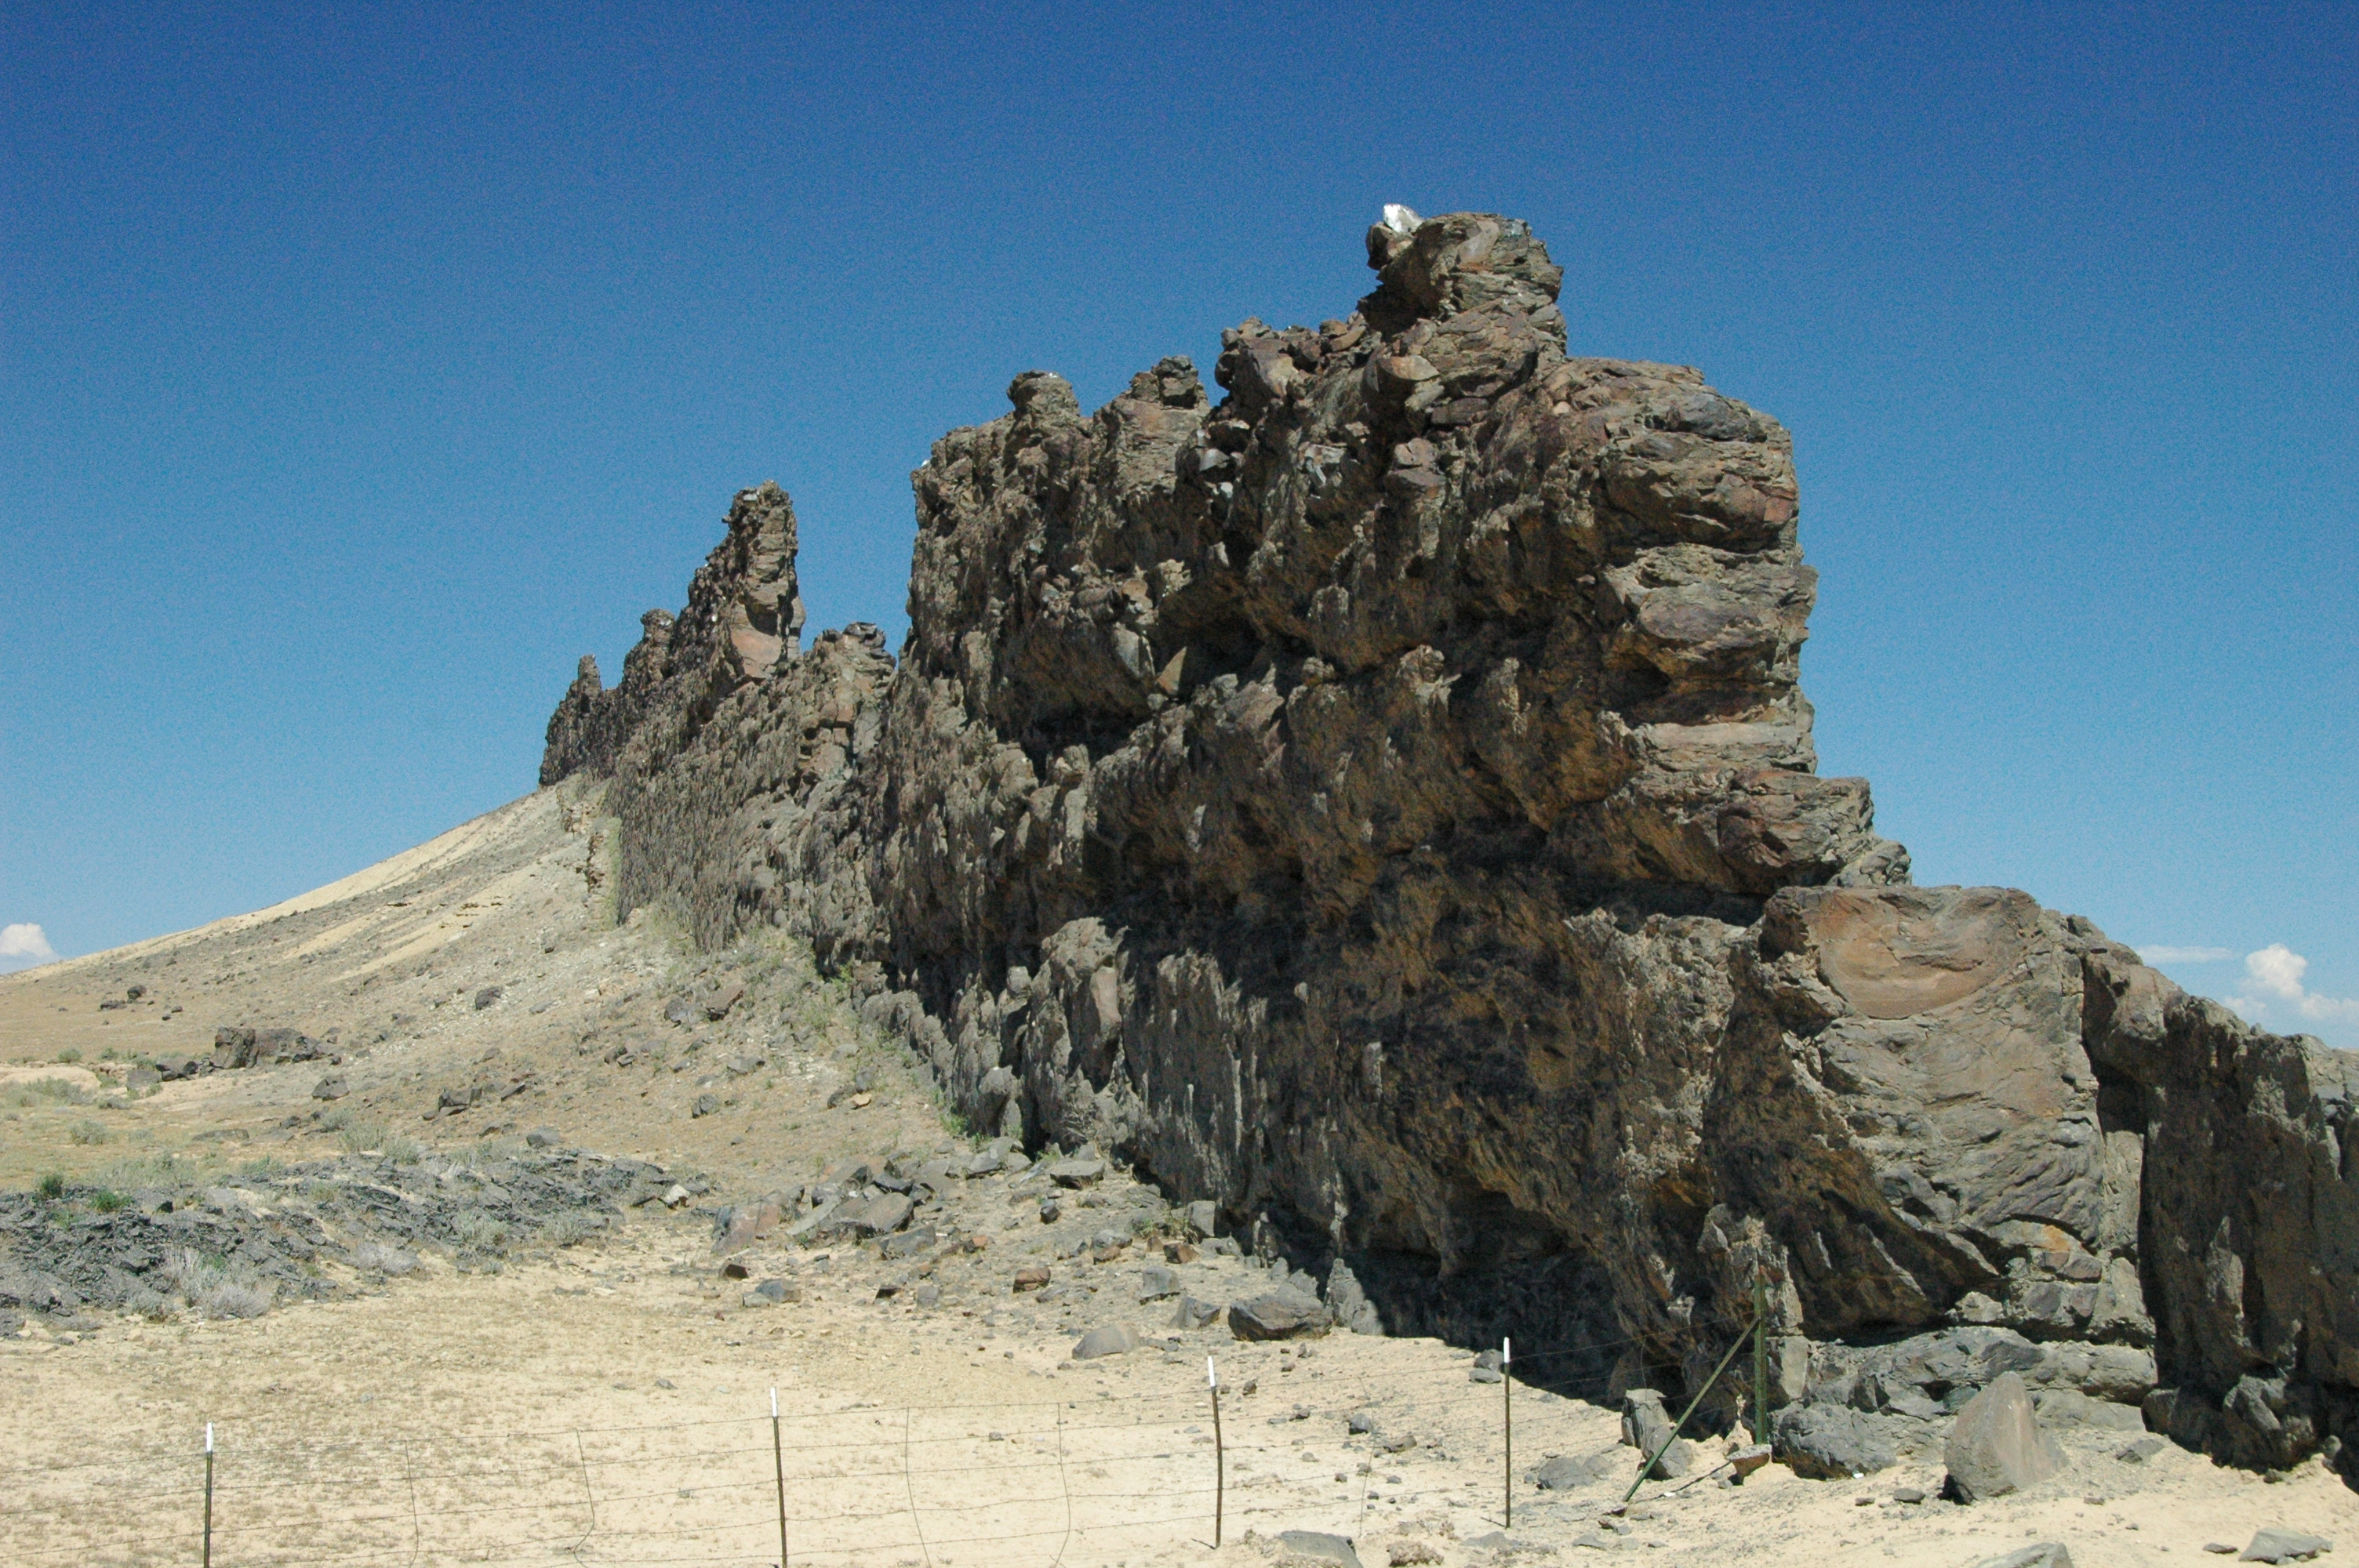
\includegraphics[width=1\linewidth]{obrazky/sopky/zila}
	\caption{Pravá žíla tvořená lamprofyrem. Stará 27-32 miliónu let. (Navajo Volcanic Field, New Mexico, USA). (Zdroj: James St. John https://www.flickr.com/people/jsjgeology/, CC BY 2.0, via Wikimedia Commons)}
	\label{fig:zila}
\end{figure}

\index{žíla}
\textbf{Ložní žíla} je konkordantní tabulové těleso o typické mocnosti \SIrange{10}{30}{\metre}. \textbf{Lakolit} je forma ložní žíly u které narostla její mocnost a vznikla tak klenba, což způsobilo i vyklenutí nadložních vrstev.

\begin{figure}[h]
	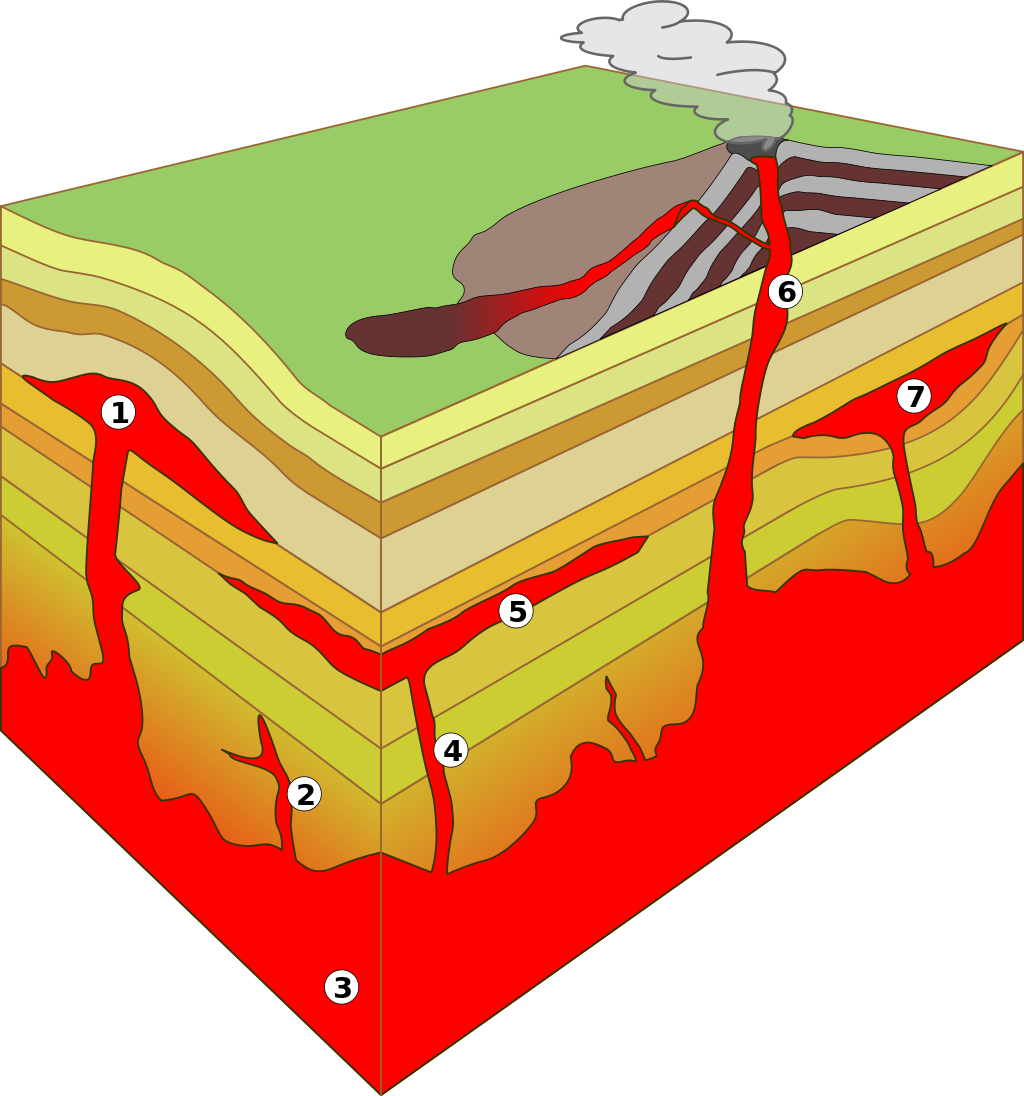
\includegraphics[width=\linewidth]{obrazky/sopky/Intrusion_types}
	\caption{Základní typy intruzí: 1. lakolit, 2. malá žíla, 3. batolit, 4. pravá žíla, 5. ložní žíla, 6. sopouch, 7. lopolit (Zdroj: Motilla, CC BY-SA 3.0 via Wikimedia Commons)}
	\label{fig:intrusion}
\end{figure}

\section{Sopky}
\subsection{Rozložení sopečné činnosti}
\index{sopky}
Sopečná činnost není rozložená rovnoměrně po zemském povrchu, ale je soustředěna hlavně na okraje litosférických desek a v místech horkých skvrn. V těchto oblastech je tak dominantním reliéfotvorným činitelem. V současné době ční nad hladinu světového oceánu okolo 600 sopek a to jak na kontinentech, tak v podobě sopečných ostrovů. Aktivních podmořských vulkánů je ale daleko víc. Udává se, že alespoň 50 000 se jich nachází na dně Tichého oceánu.

\subsection{Typy erupcí}
Podoba sopečné erupce je závislá na chemickém složení magmatu (zejména množství \ce{SiO2}), obsahu plynné složky a vody, jelikož ovlivňují jeho \textbf{viskozitu}. \emph{Kyselé (felsické) magma} (s velkým obsahem \ce{SiO2}) je viskózní, teče tedy pomalu. Neumožňuje snadný únik sopečných plynů, čímž se v sopce stupňuje tlak a často pak dochází k explozivním erupcím. Kyselá láva má malý prostorový dosah.

Málo viskózní \emph{basické (mafické) magma} (bazaltové), obsahuje cca jen 5 \% \ce{SiO2}. Materiál magmatu pochází z větších hloubek, zejména ze svrchního pláště. Toto magma je vázáno hlavně na riftové oblasti a horké skvrny. Erupce jsou mnohem klidnější. Dochází k výlevům magmatu na povrch. Díky malé viskozitě se láva roztéká do velkých ploch.

Vulkanické erupce se dělí do tří typů a to na \textbf{exhalační}, kdy do vzduchu unikají sopečné plyny. V případě, že dochází k výlevům lávy, tak je označována za \textbf{efuzivní}. V případě výbuchu hovoříme o \textbf{explozivním} typu vulkanické erupce. Do vzduchu je vyvrhován pevný materiál označovaný jako \textbf{tefra}.

\begin{table*}[]
	\setlength{\tabcolsep}{3pt}
	\footnotesize
	\begin{tabularx}{1\textwidth}{XXXXX}
		\toprule
		Typ erupce & Typ magmatu& Podoba výlevné aktivity& Podoba explozivní aktivity & Struktury a formy vytvořené okolo kráteru  \\ \midrule
		Islandská &	Basické, nízká viskozita &Rozsáhlé a silné výlevy z trhlin &Velice slabá &
		Velice rozsáhlé lávové kužely; lávové plošiny s tvorbou kuželů okolo trhlin v terminální fázi \\
		Havajská                    & Basické, nízká viskozita & Běžně tenké a rozsáhlé výlevy z centrálních sopouchů & Velice slabá & Velice rozsáhlé lávové dómy a štíty\\
		Strombolská &
		Střední viskozita; částečně kyselá, částečně bazická &
		Výlev chybí nebo jsou silné a středně rozsáhlé &
		Slabá až silná  &
		Struskové kužely a lávové proudy \\
		Vulkánská                   & Kyselé, viskózní        & Lávové proudy často chybí; případně o velké mocnosti         & Střední                      & Sypaný kužel; explozivní krátery \\
		Vesuviánská (silná Vulkánská) & Kyselé, viskózní        & Lávové proudy často chybí; silné                    & Střední až silné         & Sypaný kužel; explozivní krátery      \\
		Plinijská (extrémně silná Vulkánská) &
		Kyselé, viskózní &
		Proudy chybí; pokud jsou, tak různých mocností &
		Velice silné&
		Rozsáhlé sopečné pumy a lapilli; bežně žádná tvorba kuželun \\
		Pélejský &
		Kyselé, viskózní &
		Dómy a/nebo krátké, mocné proudy; mohou chybět &
		Podobně jako Vulkánský typ ale s nuees ardentes &
		dómy; kužely popela a prachu\\ \bottomrule
	\end{tabularx}
	\caption{Typy erupcí (upraveno podle \textcite{summerfieldGlobalGeomorphologyIntroduction1999a}).}
	\label{tab:erupce}
\end{table*}


\subsection{Sopečné produkty}
\index{lávový proud}
\subsubsection{Lávové proudy}
Magma, které se dostává na zemský povrch se označuje jako láva. Podoba lávy a formy, které tvoří jsou závislé na charakteru původního. Kyselé lávy jsou velice viskózní, což zmenšuje vzdálenost na kterou mohou dotéct. Málo viskozní, bazaltové lávy snadno tečou a dostávají se tak do značných vzdáleností od místa erupce. Dalším důležitým faktorem, který ovlivňuje rychlost tuhnutí lávy, když se dostane na povrch je také mocnost lávového proudu. 
\textbf{Pahoehoe} je láva s hladkým provazovitým povrchem, který vzniká vychladnutím tenké vrtstvy na povrchu a její následnou deformací tekoucí lávou pod povrchem. Pahoehoe vzniká z lávy o nízké viskozitě. Jejím chladnutím lávy a úbytkem plynů se viskozita zvyšuje a vzniká láva typu \textbf{aa}, jejíž povrch je rozeklaný a ostrohranný.


\begin{figure}[h]
	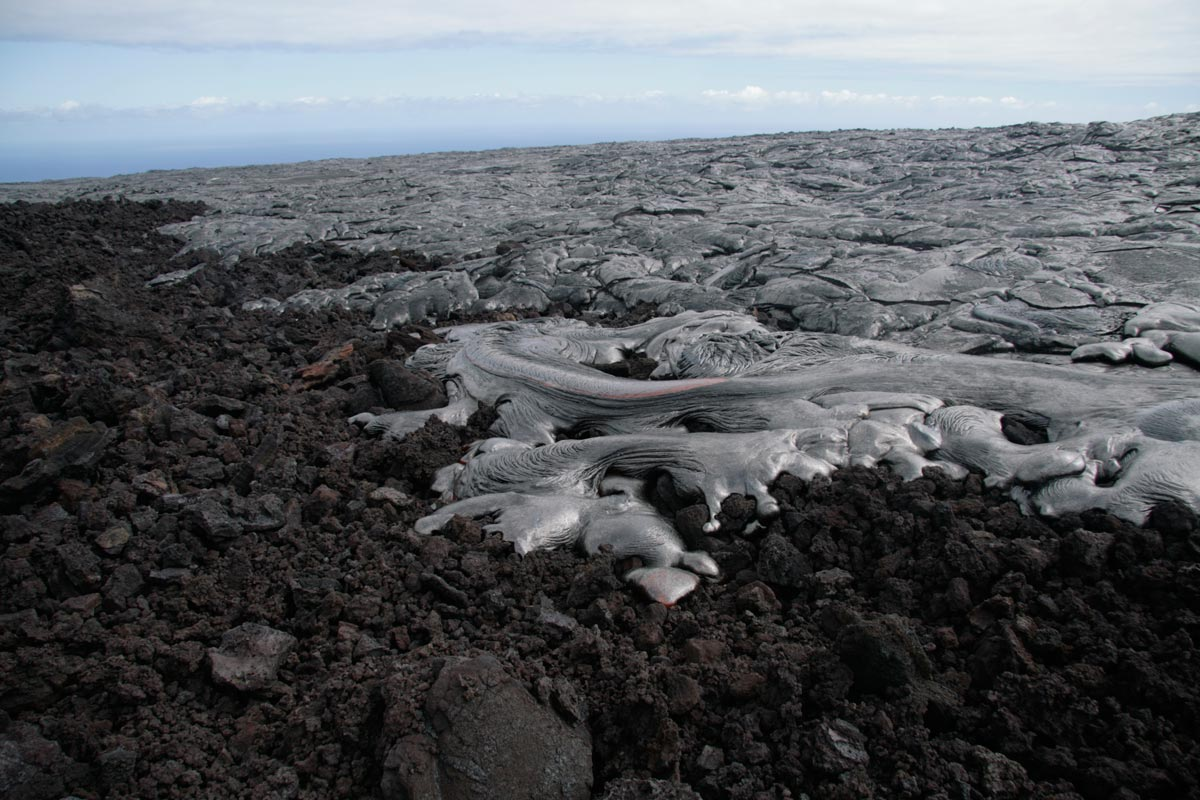
\includegraphics[width=\linewidth]{obrazky/sopky/paho_aa}
	\caption[Pahoehoe]{V popředí lávy typu aa, kterou překrývá láva pahoehoe. (Autor: USGS, veřejné dílo)}
	\label{fig:pahoe_aa}
\end{figure}

\subsubsection{Tefra}
Pyroklastický materiál, který sopky chrlí do okolí dělíme dle velikosti jednotlivých klastů. Nejjemnější je \textbf{sopečný popel}, kdy průměr částic je $<$ \SI{2}{\milli\metre}. Po zpevnění je nazýván tufem. Větší částice o průměru \SIrange{2}{64}{\milli\metre} nazýváme \textbf{lapilli}. Největší pyroklastika jsou \textbf{sopečné pumy} (průměr $>$ \SI{64}{\milli\metre} (obr. \ref{fig:puma}).

\begin{figure}[h]
	\centering
	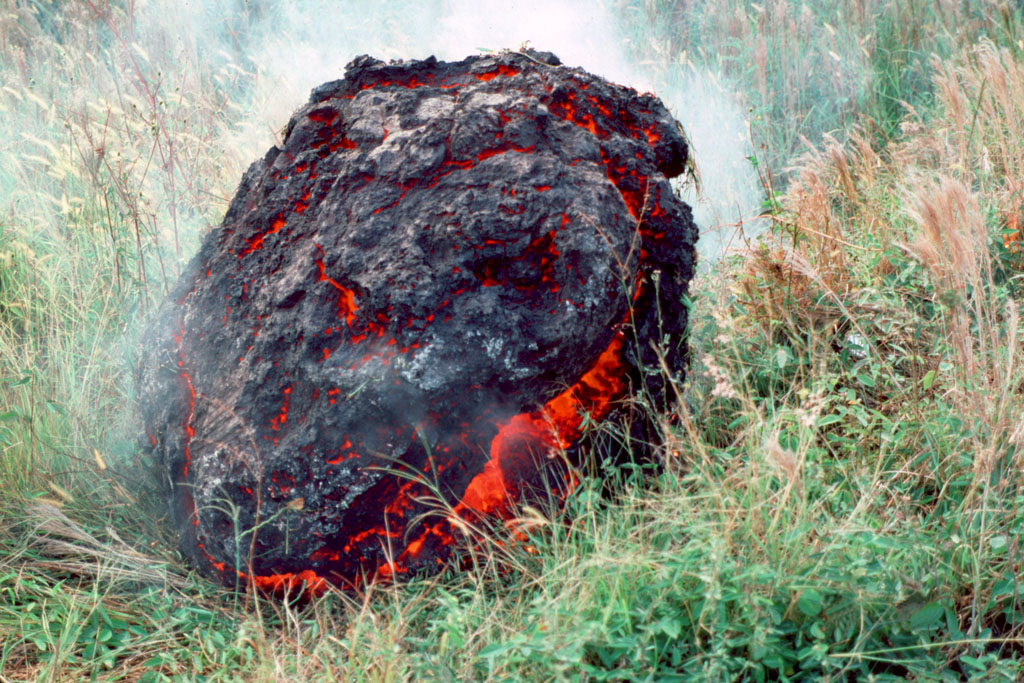
\includegraphics[width=1\linewidth]{obrazky/sopky/puma}
	\caption{Ještě žhavá sopečná puma vymrštěná ze sopky Kīlauea, Havaj (autor: J. D. Griggs, USGS, volné dílo)}
	\label{fig:puma}
\end{figure}


Zvláštním typem sopečného materiálu jsou \textbf{hyaloklastika}, která jsou spojená s erupcemi pod ledovcem. 

\subsubsection{Pyroklastický proud}
Pyroklastický proud (\textit{pyroclastic flow
}) je velice nebezpečný fenomén. Jedná se značně pohyblivou směs žhavých sopečných plynů a popela (obr. \ref{fig:pyroclastic}). Pohybuje se po sopečném svahu dolů rychlostmi, které se pohybují v rozmezí \SIrange{150}{700}{\kilo\metre\per\hour}. Teplota tekoucího materiálu je od \SIrange{100}{1100}{\celsius}.

\begin{figure}[h]
	\centering
	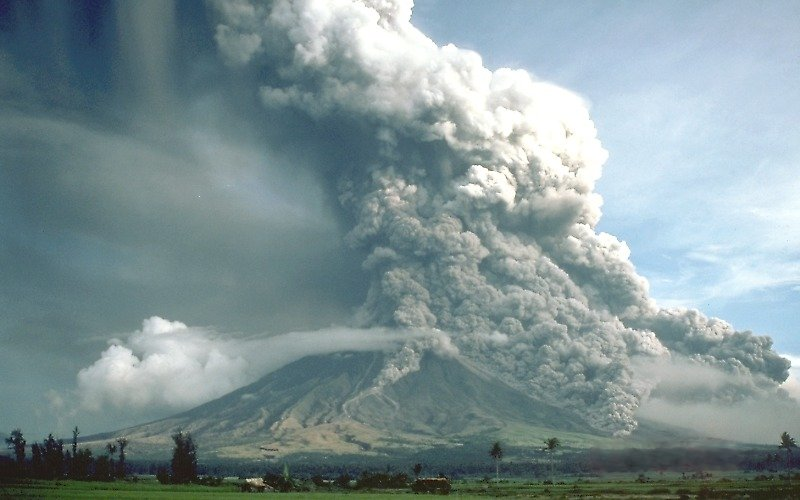
\includegraphics[width=1\linewidth]{obrazky/sopky/pyroclastic}
	\caption{Pyroklastické mračna tekoucá po úbočí sopky Mayon, Filipíny, 1984 (Autor:  C.G. Newhall, USGS)}
	\label{fig:pyroclastic}
\end{figure}


\subsection{Typy sopek}
\emph{Sypaný kužel} (tufová sopka) má podobu kužele s kráterem uprostřed, který je tvořena sopečným popelem,  struskou. Výška sypaných kuželů je zpravidla do \SI{300}{\metre}. Sypané kužely se často vyskytují ve skupinách případně v podobě parazitických sopouchů. Sypané kužely vznikají rychle (během jedné erupce -- monogenetické). 

\emph{Extruzinví sopky} neboli výtlačné kupy vznikají intruzí lávy. Kupy vzniklé vytlačením na povrch z kráteru se označují jako \emph{hornitos}. Složité výtlačné kupy, které vnzikají jako intruzivní klenby a následně roztaví nadloží se nazývají \emph{tholoidy}.

\emph{Maary} (Obr. \ref{fig:maar}) jsou malé a mělké krátery. Vznikají silnými explozemi při nadměrné produkci plynů. Mají většinou konkávní formu s nízkým obvodovým lemem ze sopečného popela. Často bývají vyplněné jezery.

\begin{figure}[h]
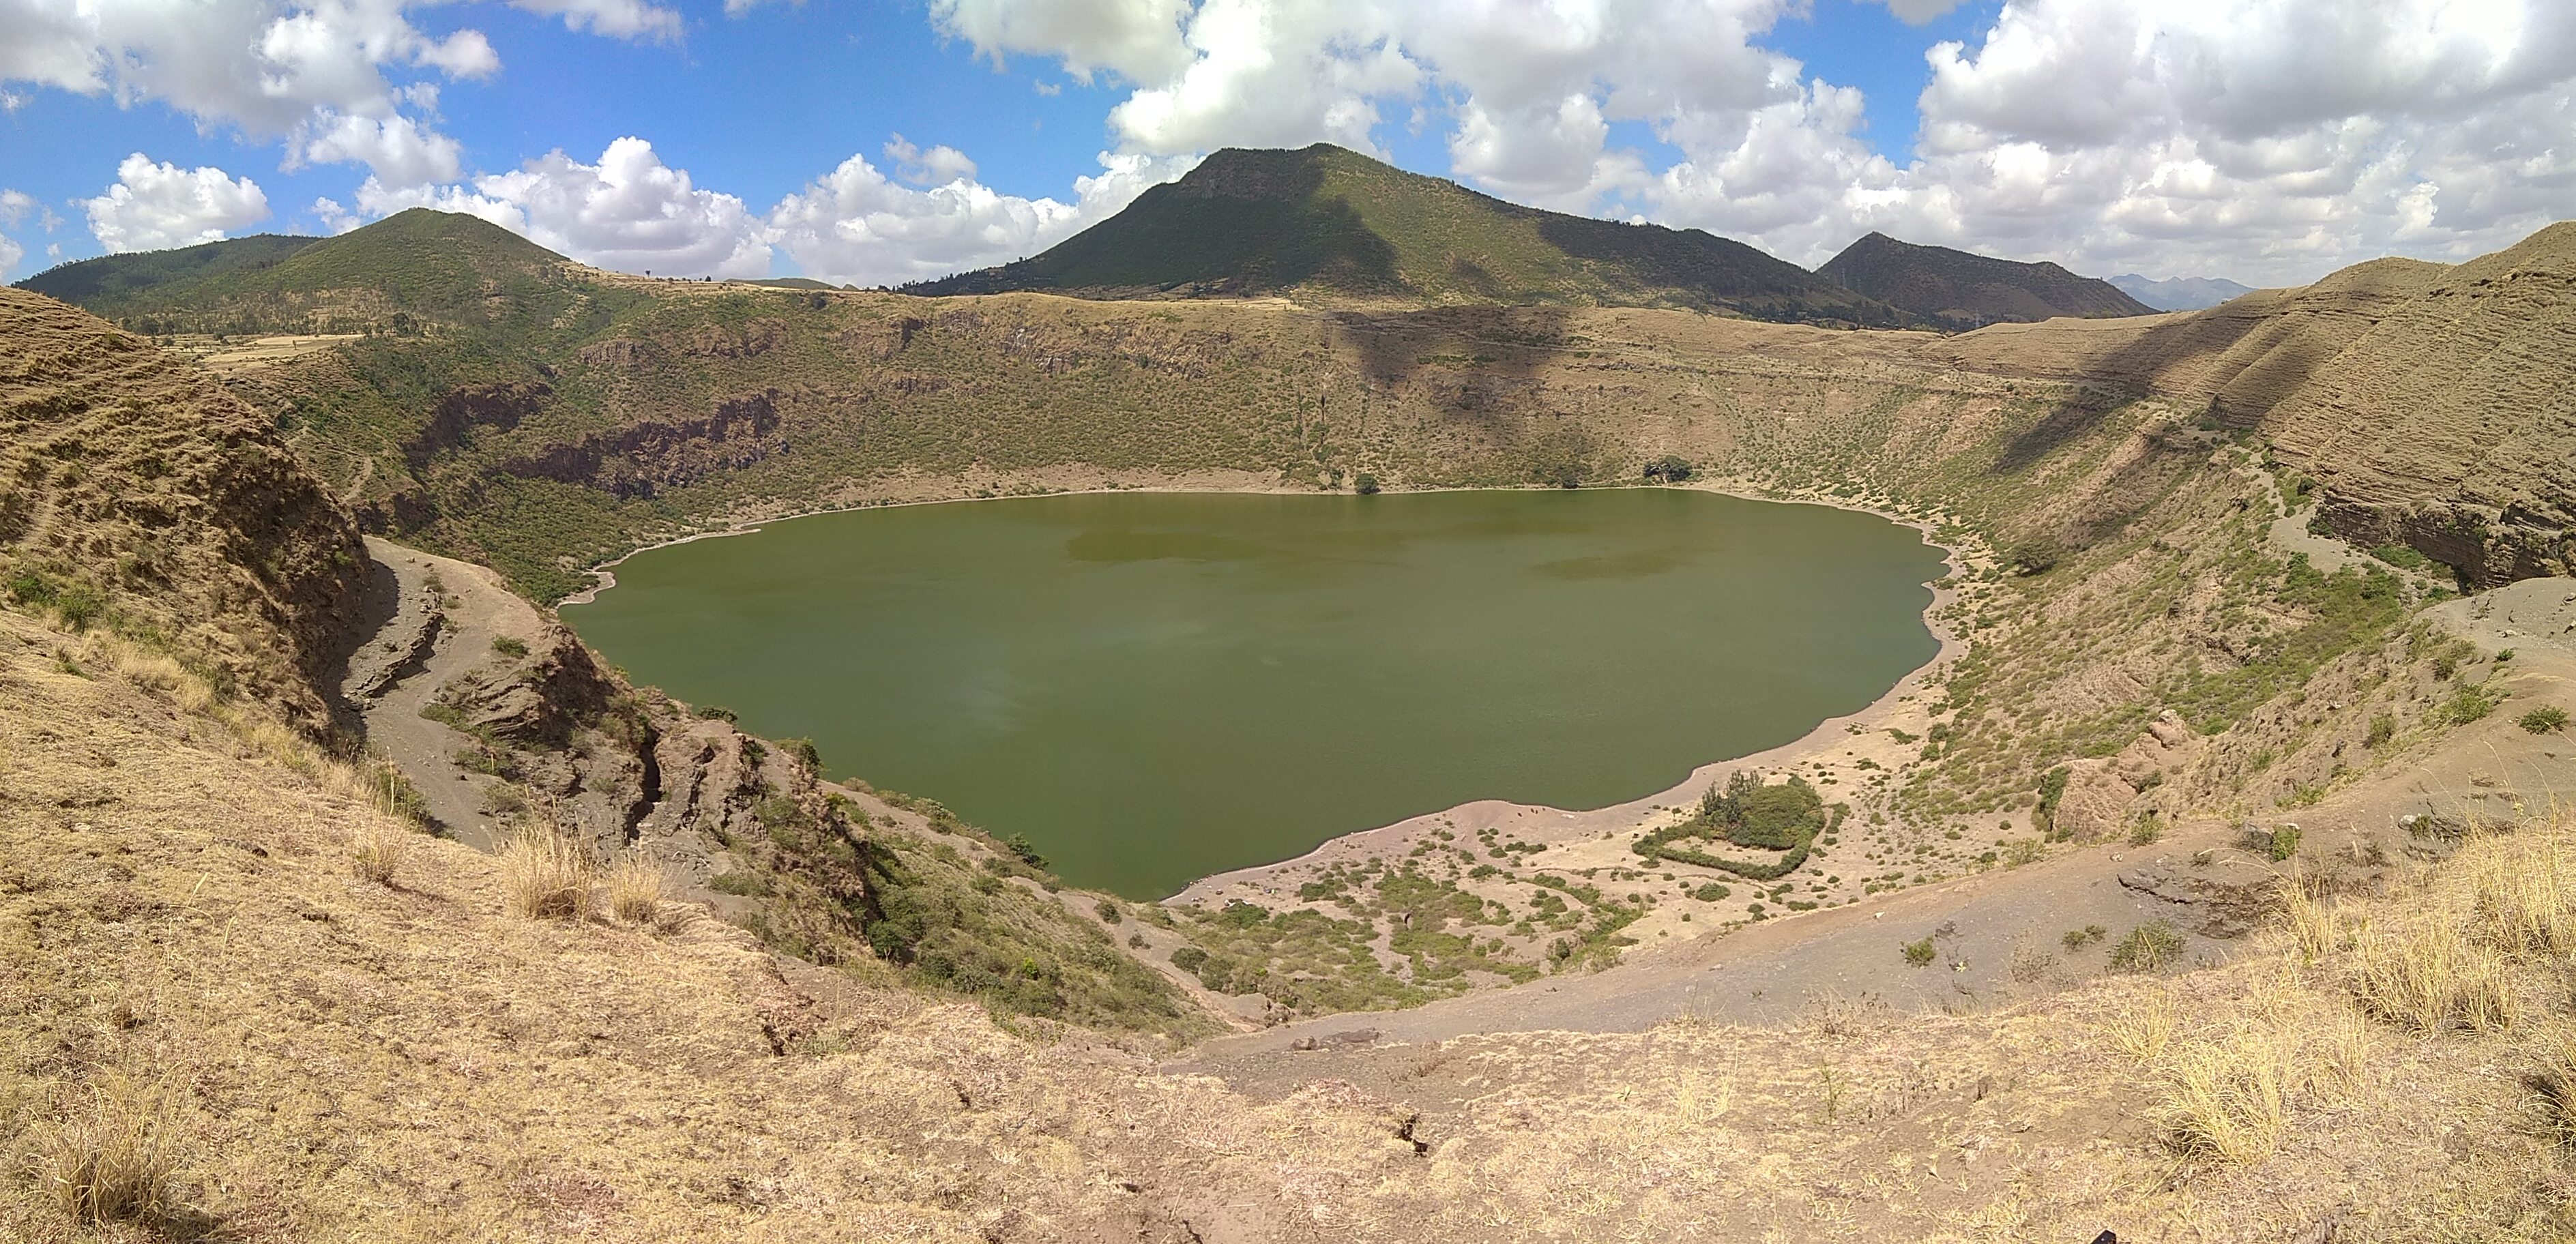
\includegraphics[width=\linewidth]{obrazky/sopky/maar}
\caption{Maar v oblasti Debre Zeit, Etiopie, Východoafrická riftová zóna (Autor: Giacomo Corti (distributed via imaggeo.egu.eu).}
\label{fig:maar}
\end{figure}

\emph{Stratovulkány} jsou nejběžnějším typem sopky. Je to smíšená sopka. Kužel stratovulkánu je tvořen ze střídajících se vrstev lávy a tefry (obr. \ref{fig:stratovulkan_rez}). Stratovulkány jsou tedy polygenetické. Na svazích se často nachází parazitické krátery. Pak hovoříme o tzv. složených stratovulkánech. 

\begin{figure}[h]
	\centering
	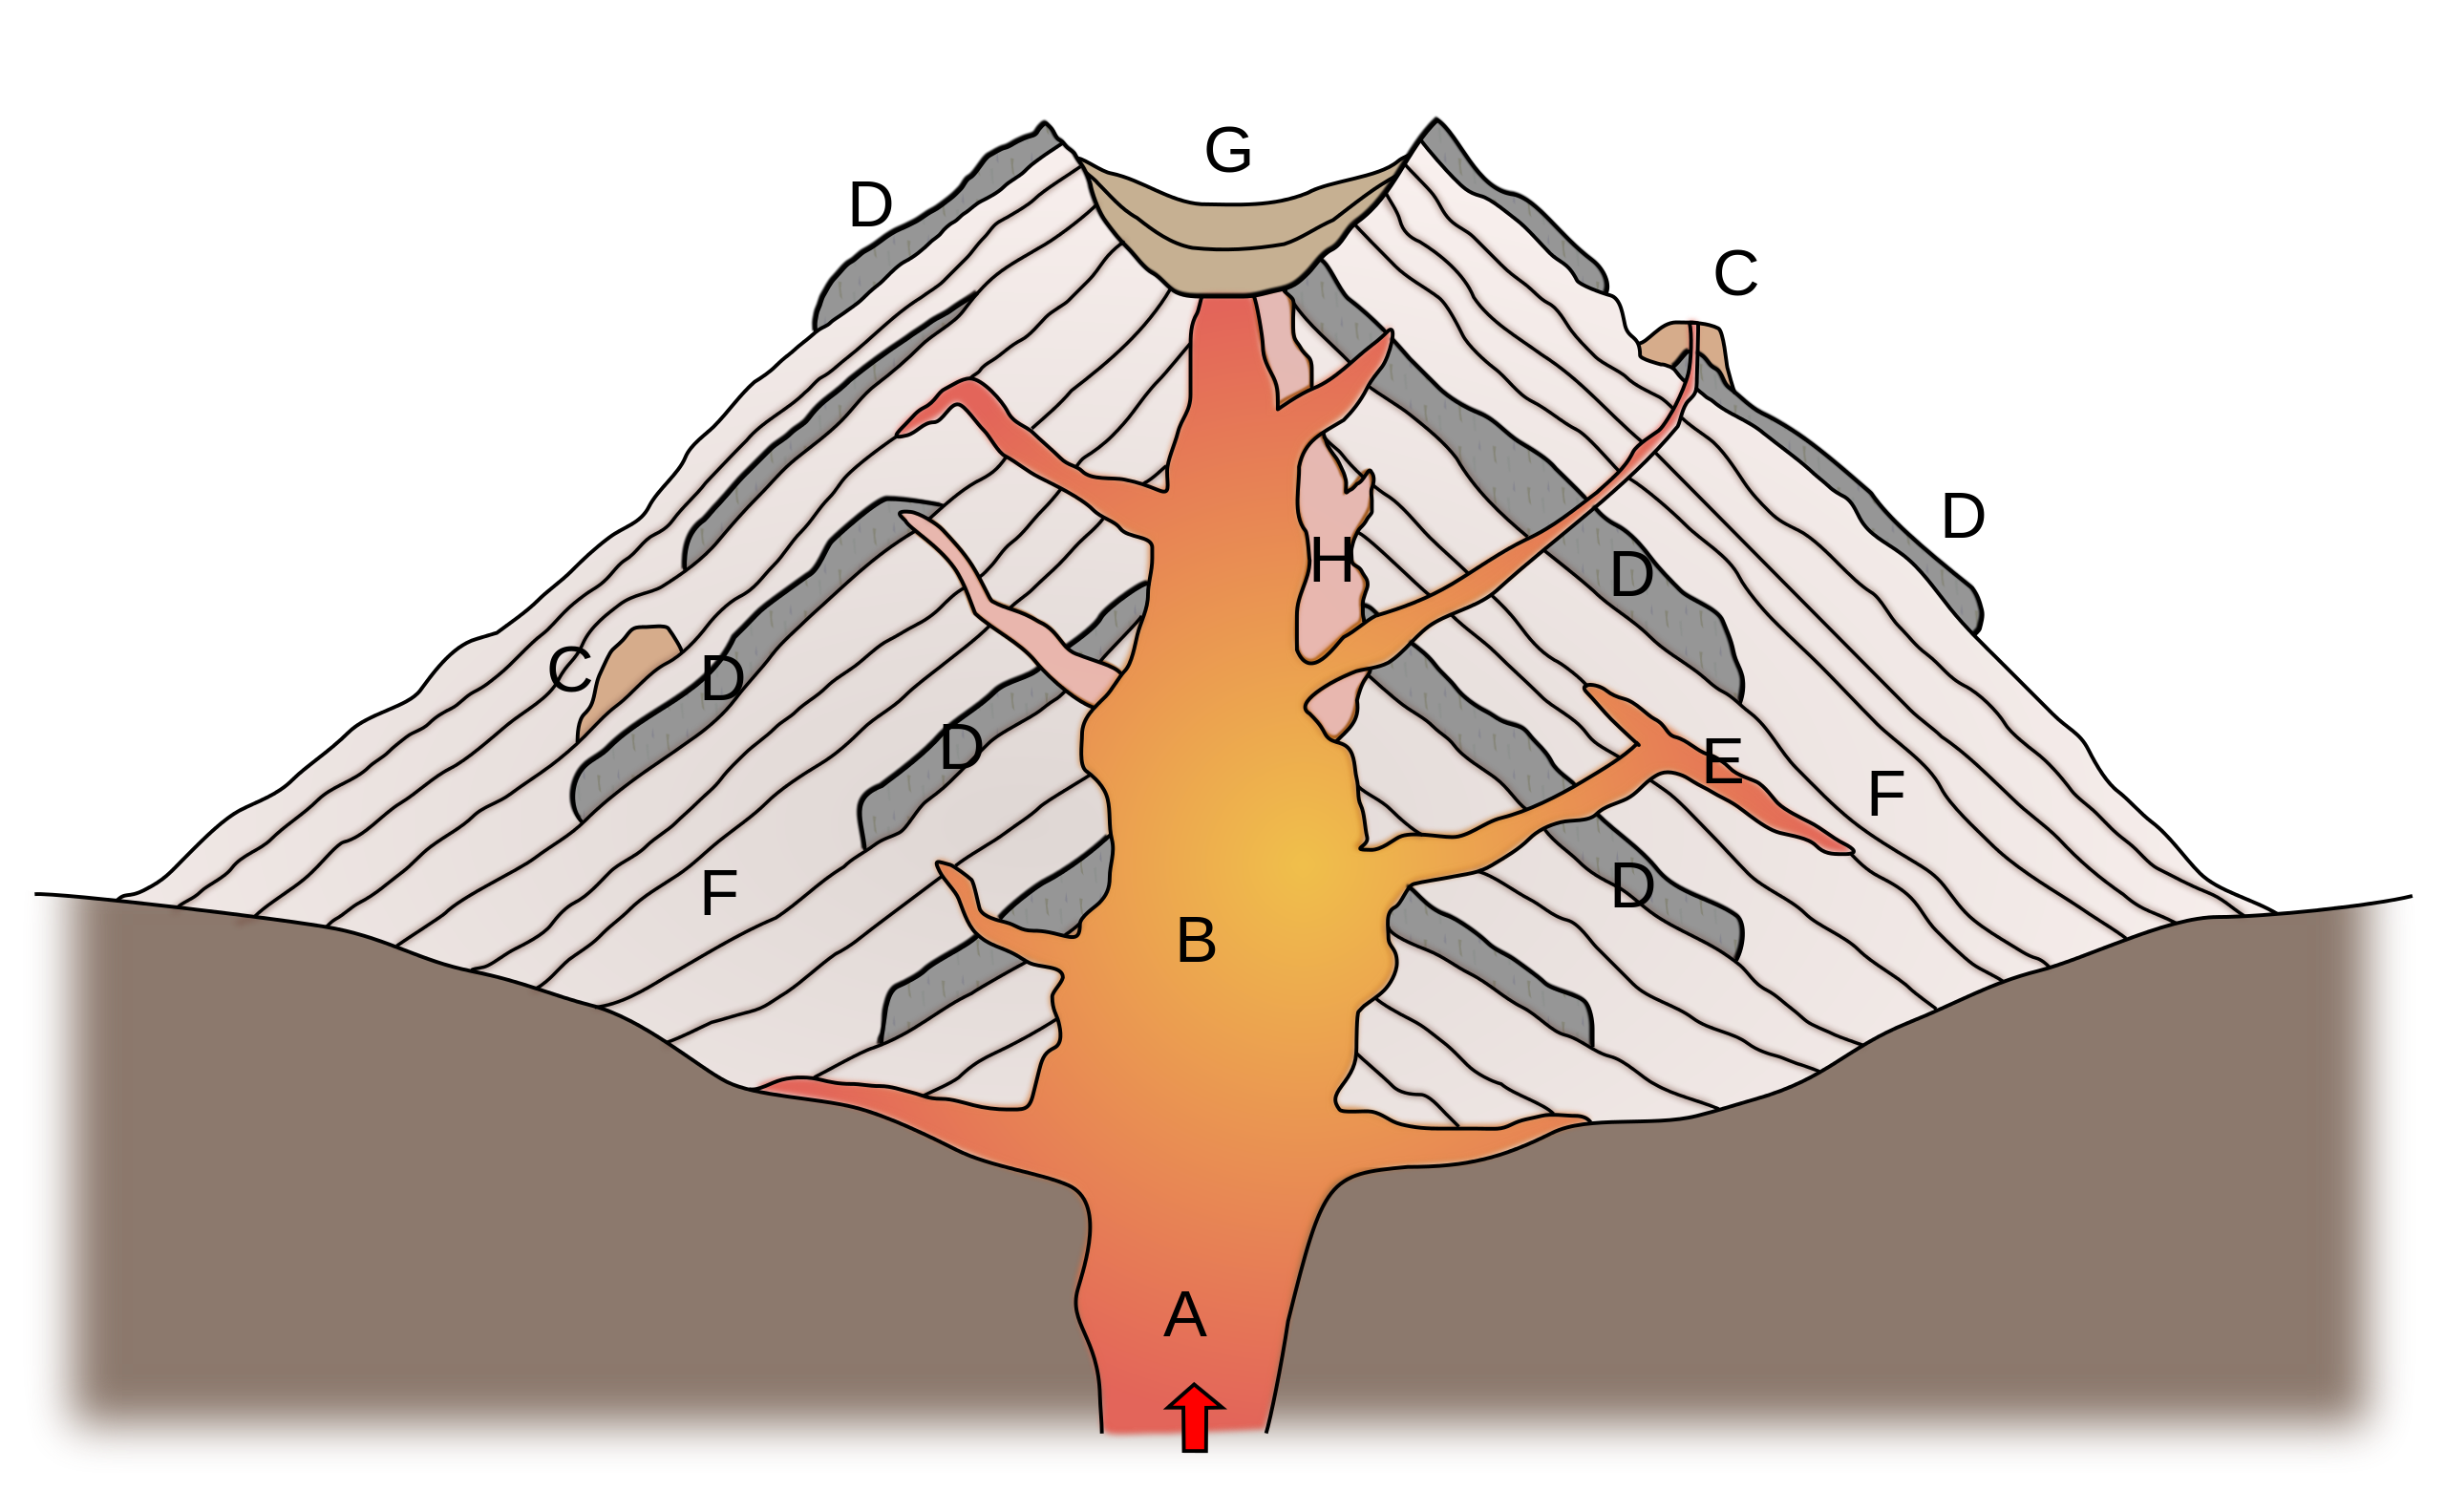
\includegraphics[width=1\linewidth]{obrazky/sopky/Stratovolcano_cross-section.svg}
	\caption{Schematický řez stratovulkánem. A: magma stoupá z magmatického krbu centrálním sopečným komínem (B); C: parazitický kráter a pyroklastický kužel na svahu stratovulkánu; D: lávový proud; E: ložní (nepravá) žíla; F: akumulace pyroklastik; G: kráter a jeho výplnň; H: starý komín (Autor: Woudloper, CC BY-SA 3.0, via Wikimedia Commons)}
	\label{fig:stratovulkan_rez}
\end{figure}




\begin{figure}[h]
	\centering
	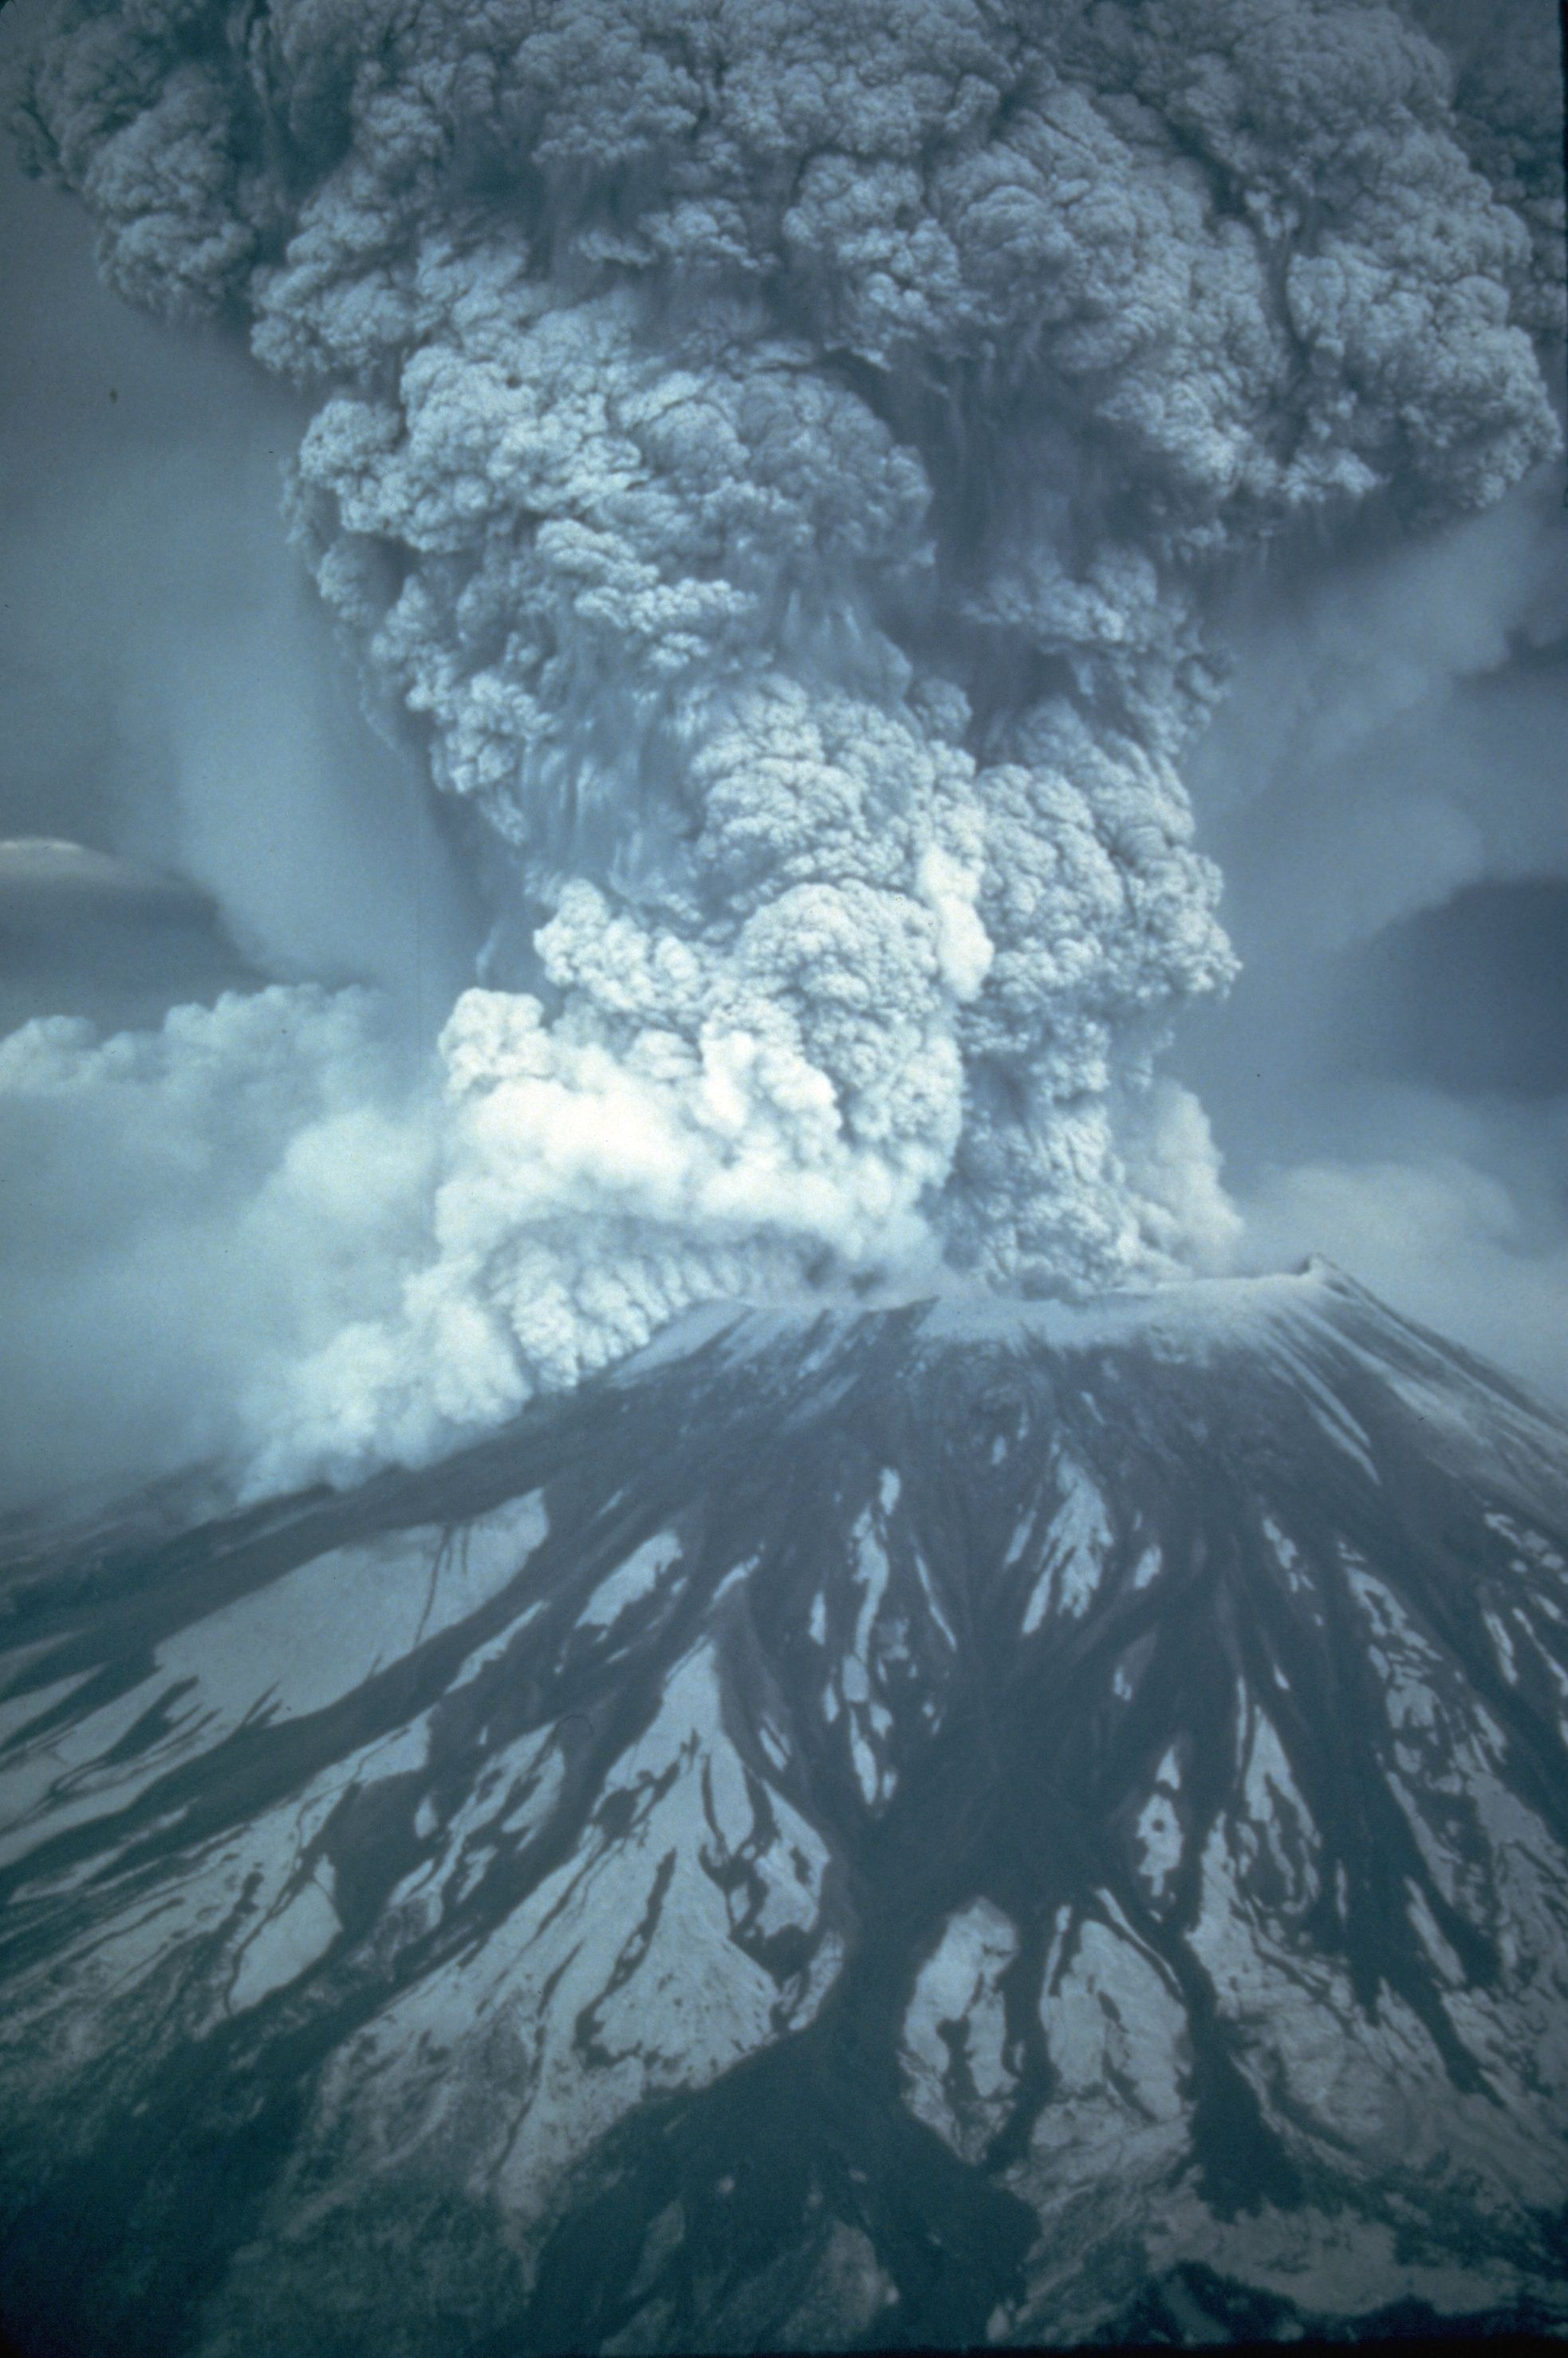
\includegraphics[width=\linewidth]{obrazky/sopky/st_helen}
	\caption{Výbuch sopky Mount St. Helens (Autor: Austin Post, volné dílo)}
	\label{fig:sthelen}
\end{figure}

Vůbec nejrozsáhlejší vulkanickou formou jsou \textbf{štítové sopky}. Mohou nabývat dvou forem: centrální sopka s jedním kráterem kruhového charakteru. Druhá podoba je lineární sopka (tzv. eldgjá). Štítové sopky mají širokou základnu, sklon svahů je velice mírný (většinou $<$\SI{10}{\degree}). Dosahují ale velkých nadmořských výšek. Největší štítové sopky na Zemi lze nalézt na Havaji. Mauna Loa (obr. \ref{fig:maunaloa}) a Mauna Kea dosahují výšky \SI{4000}{\metre} nad mořem. Avšak jejich základna o šířce přes \SI{200}{\kilo\metre} se nachází v hloubce více jak \SI{5000}{\metre}. Největší štítová sopka ve Sluneční soustavě se nachází ale na Marsu. Olympus Mons ční do výšky \SI{26}{\kilo\metre}

\begin{figure*}[h]
	\centering
	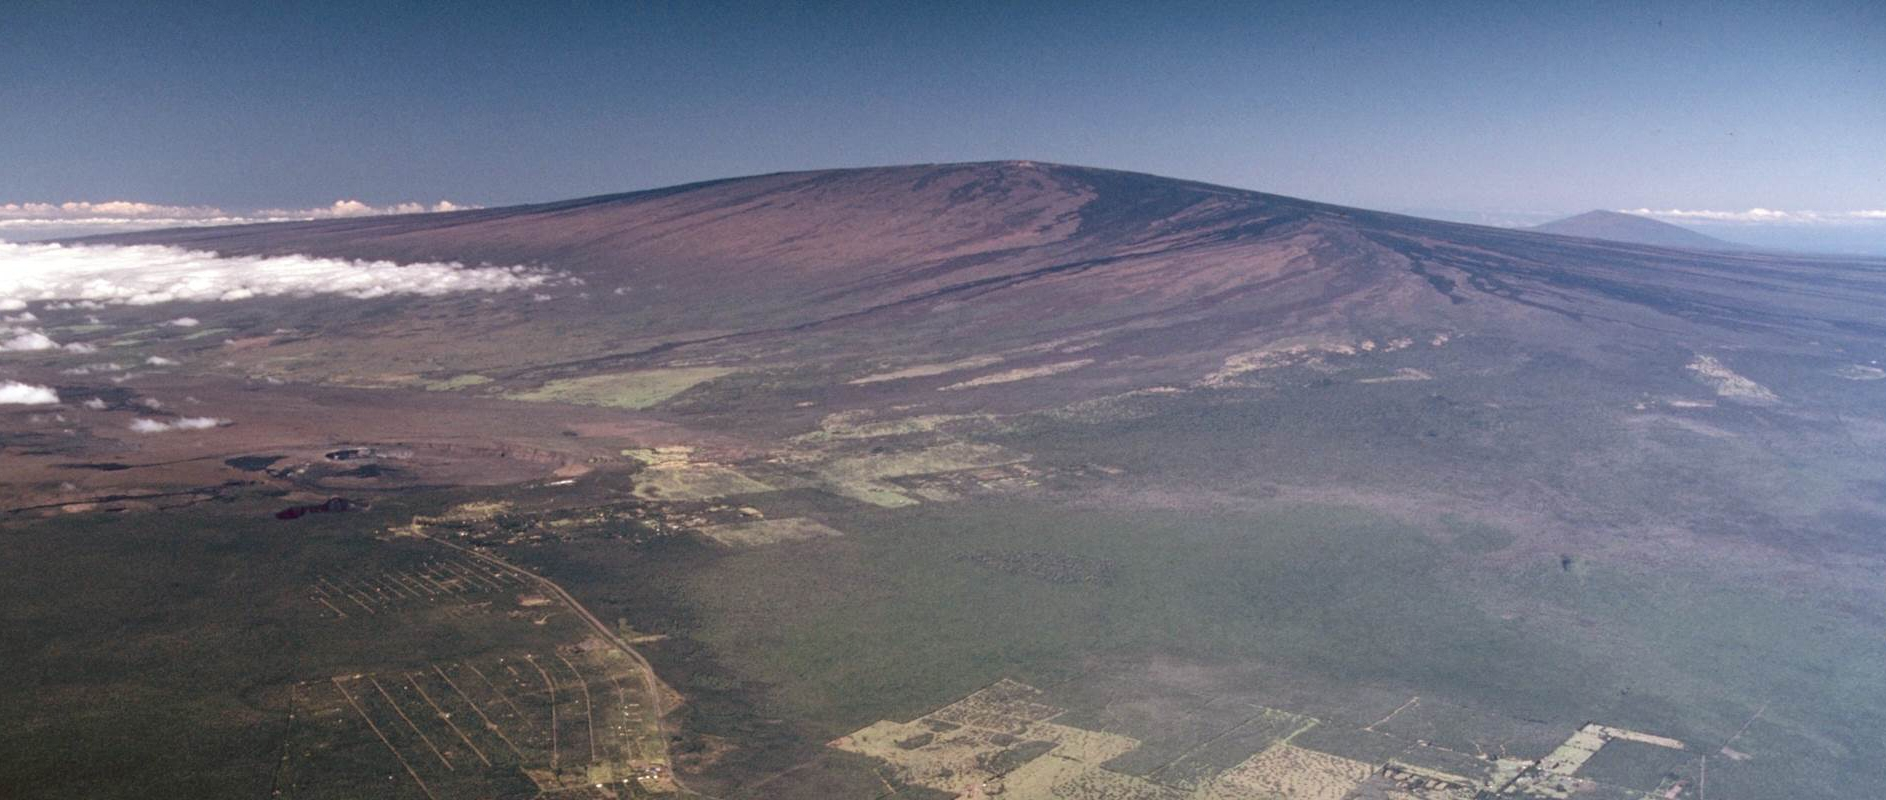
\includegraphics[width =1\textwidth]{obrazky/sopky/mauna_loa}
	\caption{Štítová sopka Mauna Loa, největší aktivní sopka na Zemi. Fotografie z roku 1985the largest active volcano on Earth. (Credit: J.D. Griggs, USGS, volné dílo)}
	\label{fig:maunaloa}
\end{figure*}

\textbf{Kaldery} jsou rozsáhlé krátery, které jsou geneticky spojené s vulkanismem. Dělíme je na explozivní -- vzniklé výbuchem již existujícího vulkánu a subsidenční, které vznikly poklesem povrchu nad vyprázdněným magmatickým krbem. 

\begin{figure*}[h]
	\centering
	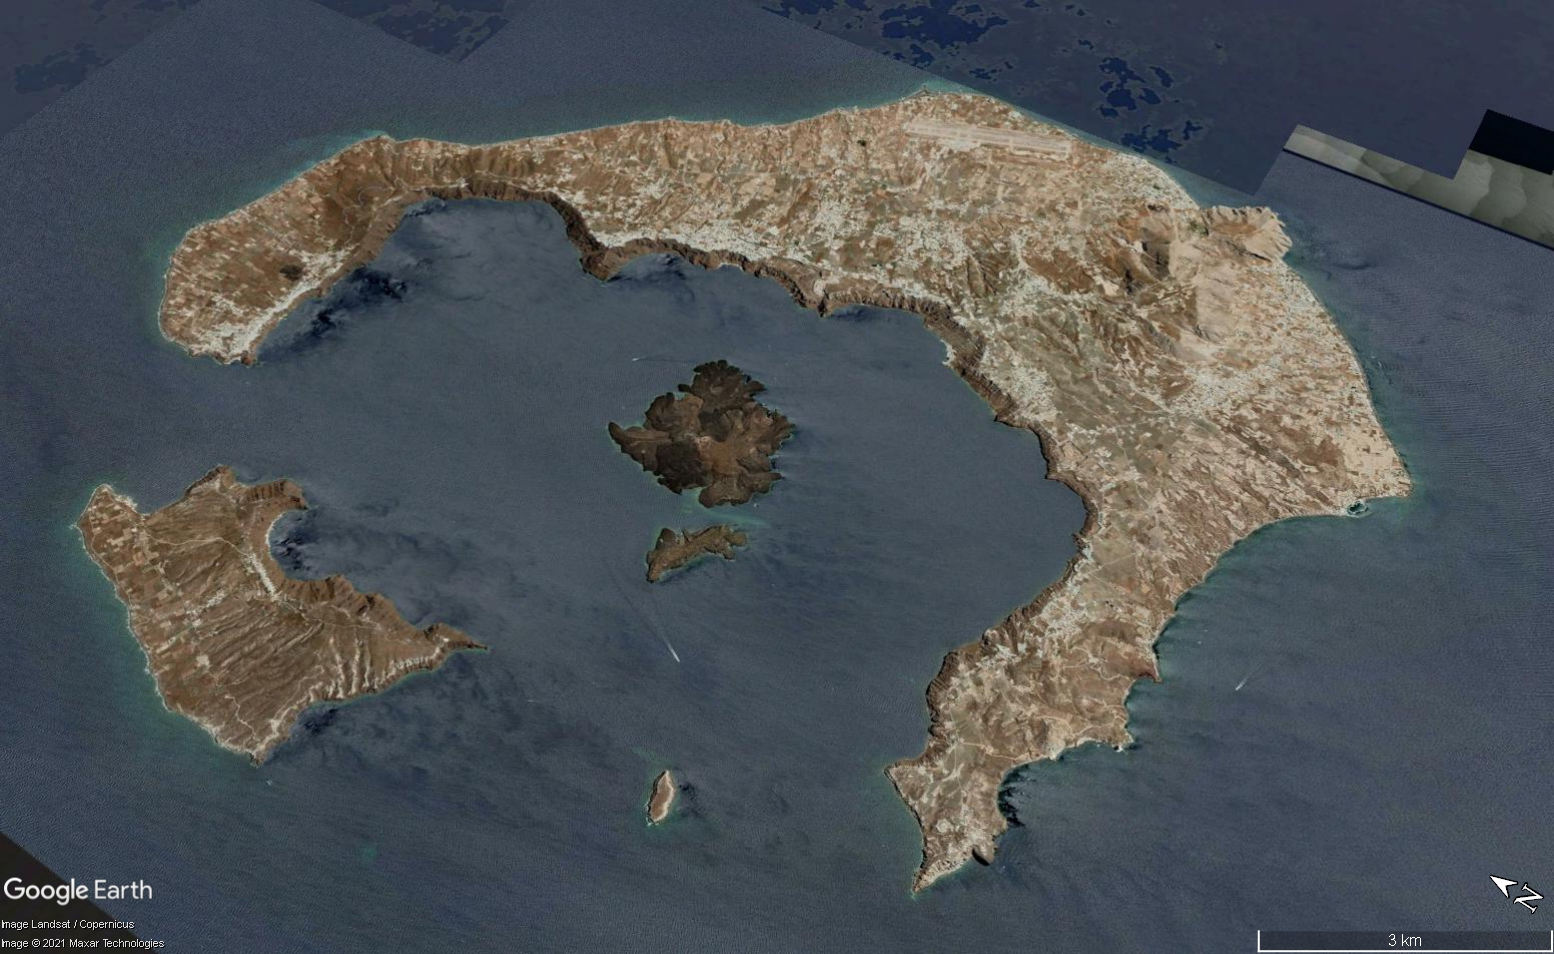
\includegraphics[width =\linewidth]{obrazky/sopky/santorini}
	\caption{Sopečná kaldera, ostrov Santorini, Řecko (Google Earth)}
	\label{fig:santorini}
\end{figure*}

\textbf{Trappy} jsou lávové pokryvy, které pokrývají rozsáhlé oblasti v plochém terénu. Známé jsou tzv. Dekkánské trapy v západní Indii (Obr. \ref{fig:trapy}), které jsou jedním z nejrozsáhlejších vulkanických těles na světě. V současné době je jejich plocha přibližně \SI{500000}{\kilo\metre\squared}. 

\begin{figure*}[h]
	\centering
	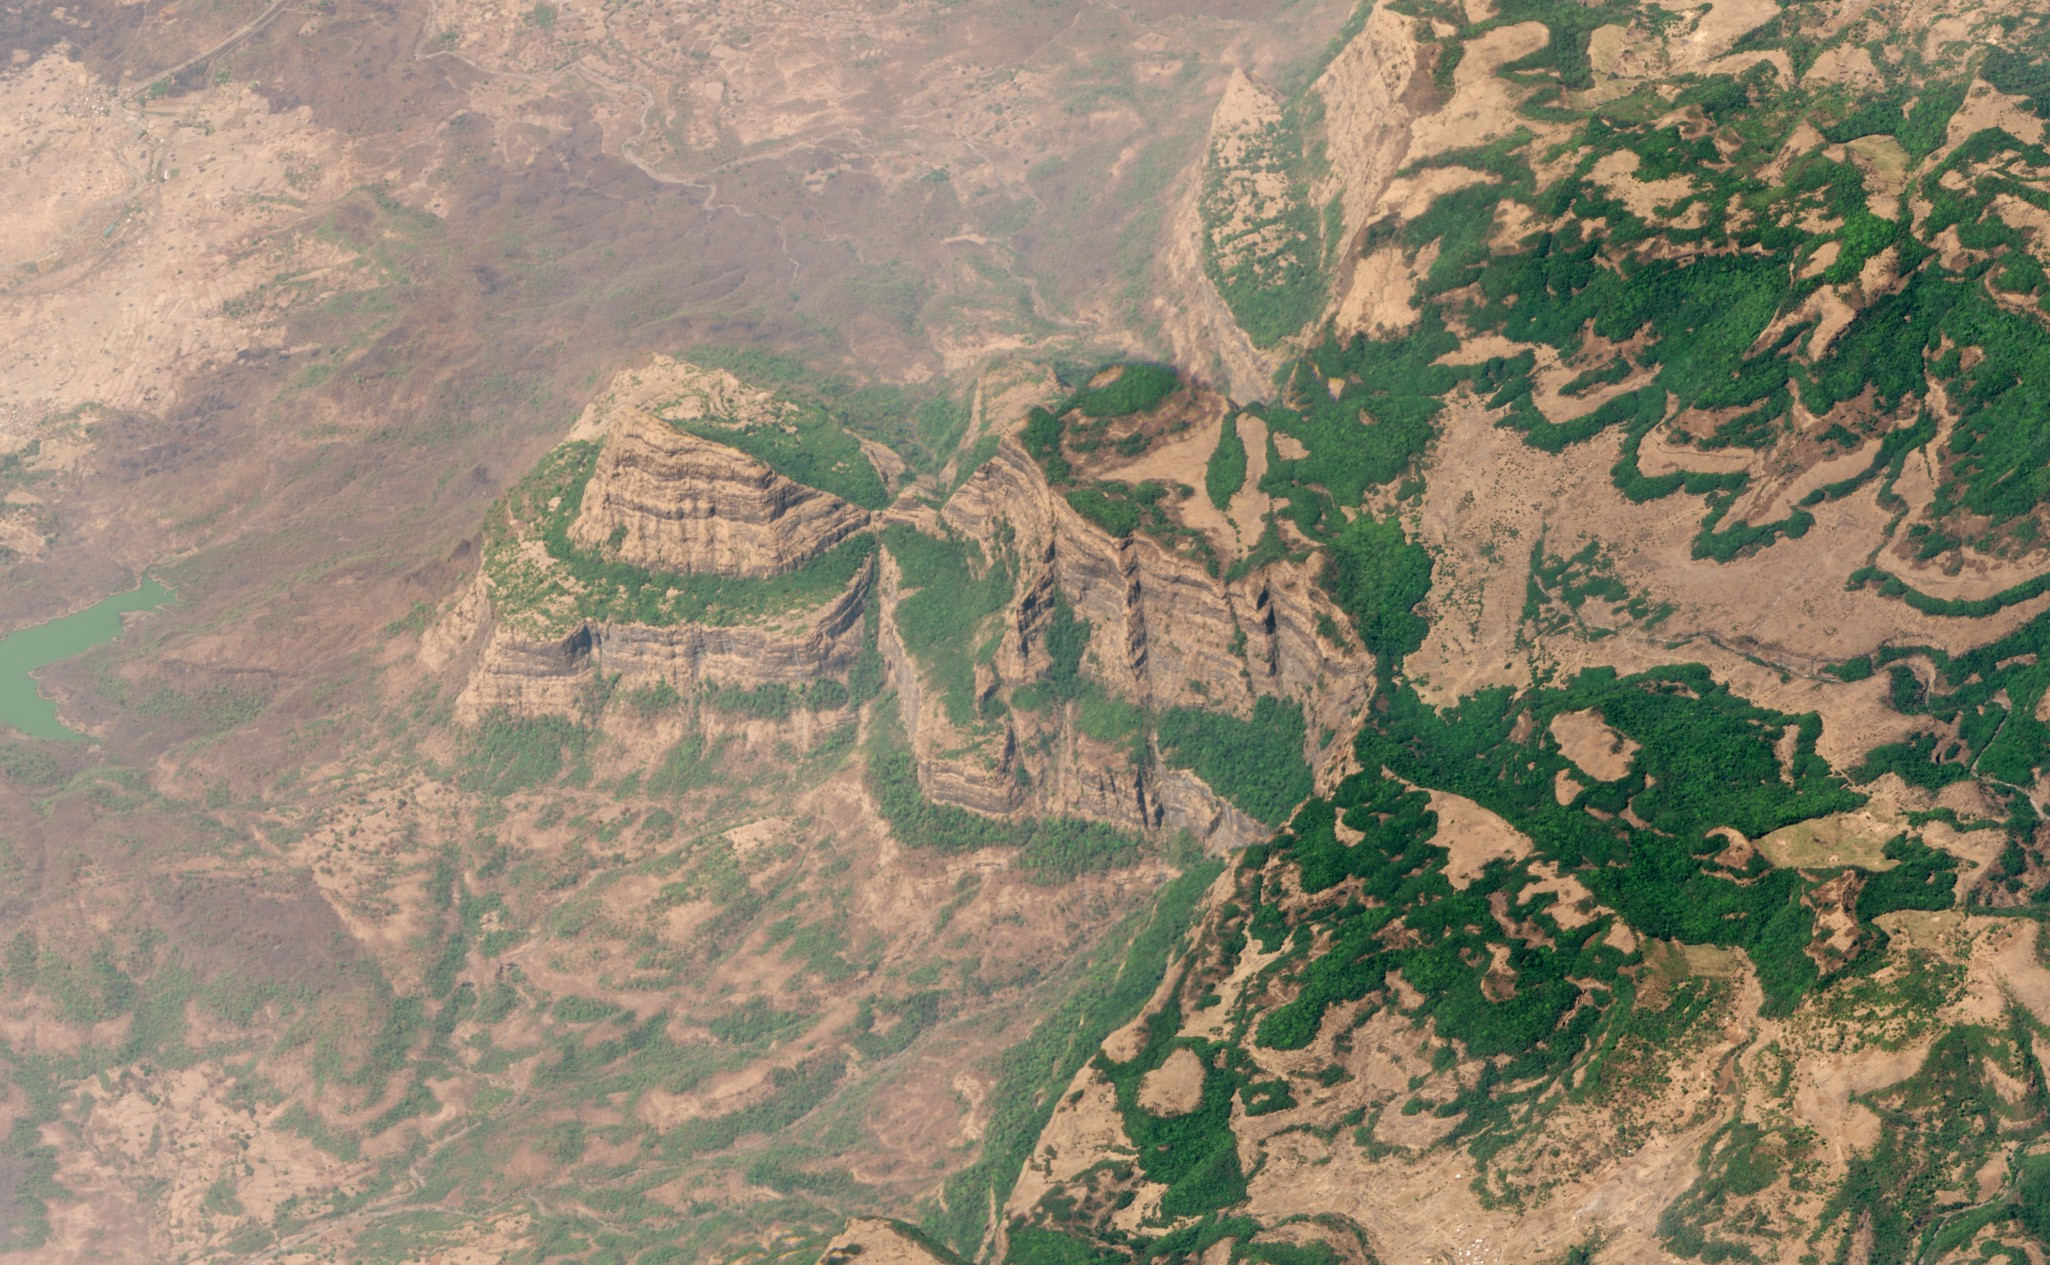
\includegraphics[width=\linewidth]{obrazky/sopky/trapy}
	\caption{Dekkánské trapy (zdroj: By Planet Labs, Inc - \url{https://medium.com/planet-stories/earths-wonders-like-you-ve-never-seen-them-before-ac9e2f39aa56}, CC BY-SA 4.0)}
	\label{fig:trapy}
\end{figure*}

\newpage
\onecolumn
\begin{boxotazky}{Kontrolní a klíčové otázky, na které bychom měli znát odpověď}
	\begin{itemize}
		\item 
		\item 
		
	\end{itemize}
\end{boxotazky}

\begin{boxslovnik}{Další klíčové pojmy k zapamatování}
	aaa & adfasd \\
	
\end{boxslovnik}
\twocolumn